\subsubsection{Agenten RTE}
\label{sec:AgentRTE}
Auf der nächsten Hierarchieebene über den Interfaces liegt die Laufzeitumgebung der Agenten (AgentRTE). Es ist die erste plattformunabhängige Ebene über den Interfaces und dem Betriebssystem. Vergleicht man die Implementation für STASH-Controller und \textsc{Mica}z-Module, unterscheidet sich das AgentenRTE lediglich im Prozessmodell der Agenten, das abhängig vom Betriebssystem ist: Während die STASH-Controller mit dem MSP430-Mikrocontroller auf SYS/BIOS mit präemptivem Scheduling stetzen, läuft auf den \textsc{Mica}z-Modulen ein nicht-präemptives Contiki-System. Die Agenten auf den Stash-Controllern werden daher jeweils durch einen eigenen Prozess repräsentiert, während es auf den \textsc{Mica}z-Modulen einen gemeinsamen Prozess gibt, der Agenten über Funktionszeiger aufruft. Wir gehen hier nur auf die Implementierung auf den \textsc{Mica}z-Modulen ein.

Neben dem Aufruf der einzelnen Agenten ist das AgentenRTE auch für das Registrieren und Terminieren der Agenten und den Austausch beziehungsweise die Verteilung von Nachrichten verantwortlich.

\paragraph{Verwaltung der Agenten}\mbox{}\\
Agenten werden mit ID und Typ registriert. Nach Konvention bekommt dabei der Plattform-Agent stets die ID des Moduls, der Order-Agent eine um eins erhöhte ID und der Routing-Agent eine um zwei erhöhte ID. Hat Beispielsweise das Modul die ID \textit{0x0110}, so hat der Plattform-Agent ebenfalls die ID \textit{0x0110}, der Order-Agent die ID \textit{0x0111} und der Routing-Agent schließlich die ID \textit{0x0112}. Die Registrierung dieser Agenten erfolgt in der Main-Methode des Systems. Die Nummerierung der Paket-Agenten ist unabhängig von dieser Konvention, allerdings muss darauf geachtet werden, dass ihre IDs nicht mit den übrigen Agenten übereinstimmen.

Registrierte Agenten werden in ein Array aus Agenten-Strukturen eingetragen und dort verwaltet.
\autoref{lst:agentstruct} zeigt die Agenten- und Agenten-Callback-Strukturen. Außerdem wird einmalig ihre Init-Methode aufgerufen.

Bei der Ausführung wird nun bei jedem Prozessaufruf des Agenten-Prozesses eine Zählervariable erhöht, die jeweils die Main-Methode des nächsten Agenten aufruft. Da  Contiki ein nicht-präemptives Scheduling nutzt, dürfen die Agenten nicht blockieren, sondern müssen die Kontrolle an den Haupt-Prozess zurückgeben, sprich die Main-Methode muss terminieren.

\lstinputlisting[language=C, style=customc, captionpos=b, caption={Agenten Strukturen in C}, label=lst:agentstruct]{src/flow/lst/agent_struct.lst}

\paragraph{Austausch von Nachrichten}\mbox{}\\
Der Austausch von Nachrichten und damit die Kommunikaion zwischen Agenten ist unerlässlich in einem Multiagentensystem. Auch diese Aufgabe kommt dem AgentenRTE zu. Die Laufzeitumgebung prüft den Empfänger einer Nachricht und übergibt sie schließlich an den richtigen Agenten. Der Aufbau einer solchen Agenten-Nachricht wird durch eine Struktur beschrieben, die in \autoref{lst:commsg} abgebildet ist. Der Kopf einer Nachricht ist demnach 15 Byte groß, die Nutzdaten können bis zu 26 Byte betragen.

\lstinputlisting[language=C, style=customc, captionpos=b, caption={Struktur einer Agenten-Nachricht in C}, label=lst:commsg]{src/flow/lst/message_struct.lst}

Sendet ein Agent eine solche Nachricht, übergibt er sie dem AgentRTE. Dieses prüft, ob sich der Empfänger-Agent auf dem eigenen Modul befindet. Ist das der Fall, wird die Nachricht in der Warteschlange für eingehende Nachrichten gespeichert und kann dort vom Empfänger abgerufen werden. Wenn der Agent nicht auf der Plattform registriert ist, wird die Nachricht an das CommunicationInterface weitergeleitet, das sich zum die Verteilung im Netzwerk kümmert. So gelangt die Nachricht auch über die Modulgrenzen hinweg zum richtigen Agenten.

Eingehende Nachrichten werden vom CommunicationInterface an das AgentRTE weitergereicht. Dafür wird zunächst angefragt, ob sich der Ziel-Agent beziehungsweise einer der Ziel-Agenten im Falle von Gruppennachrichten auf der Plattform befindet. Ist dies der Fall wird die Nachricht in der Warteschlange für eingehende Nachrichten gespeichert.

Ein großes Problem bei Nachrichtenaustausch stellt der mit 4 KB sehr begrenzte Arbeitsspeicher der \textsc{Mica}z-Module dar. Entsprechend ist der Platz in der Warteschlange für eingehende Nachrichten begrenzt, pro Agent können nur drei Nachrichten gespeichert werden. Um den Speicher nicht überlaufen zu lassen und dadurch Nachrichten zu verlieren, wird daher das Senden von Nachrichten durch ein Token-System begrenzt. Pro Agent kann so in jedem Durchlauf nur eine Nachricht versendet werden. Nutzt ein Agent dies nicht aus, kann sein Token auf einen anderen Agenten übertragen werden. In der Praxis schränkt diese Restriktion die Agenten in ihrer Funktionalität jedoch nicht ein. Meist erfordert eine eingehende Nachricht nur eine direkt Antwort oder die Benachrichtigung eines anderen Agenten. Müssen einmal doch zwei oder mehr Nachrichten als Reaktion versendet werden, geschieht dies mithilfe von Zwischenzuständen und Flags, die beim nächsten Durchlauf aktiv werden.
%\begin{figure}[h!]
%	\centering
%		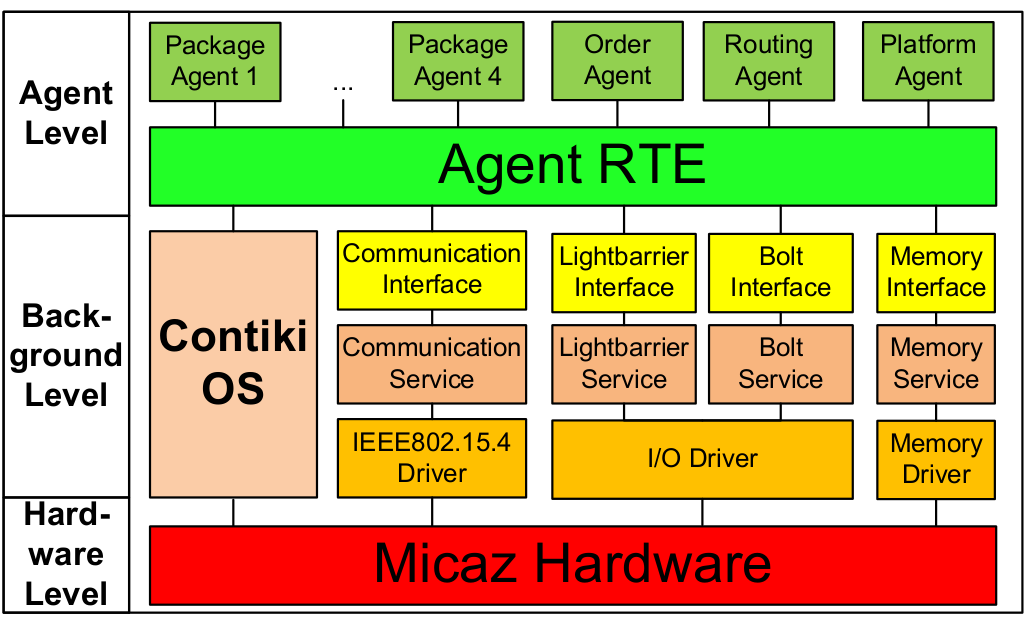
\includegraphics[width=0.9\textwidth]{ArchitekturMicazRampe.png}
%	\caption{Architektur Micaz Rampe\cite{Stasch:Hahn}}
%	\label{ArchitekturMicazRampe}
%\end{figure}
